Es folgt nun die Installation des Grundsystems. Diese hält sich größtenteils an die des ArchWiki, nur einige hardwarespezifische Änderungen, wie Grafikkartentreiber werden hier vorgenommen.\\
\\
Nach dem Bootvorgang ist man als root eingeloggt.
Lade deutsches Tastaturlayout:
\begin{lstlisting}[style=Bash]
# loadkeys de
# loadkeys de-latin1
\end{lstlisting}

\subsection{Netzwerk}
\label{subsec:network}
Ist Ethernet Netzwerkkarte geladen?
\begin{lstlisting}[style=Bash]
# ip link 
\end{lstlisting}
Wenn nein, Modul herausfinden:
\begin{lstlisting}[style=Bash]
# lspci -v | less 
\end{lstlisting}
Fehlermeldung des Moduls analysieren:
\begin{lstlisting}[style=Bash]
# dmesg | grep tg3 
\end{lstlisting}
Modul erneut laden
\begin{lstlisting}[style=Bash]
# modprobe -r tg3
# modprobe tg3
\end{lstlisting}
Verfizieren:
\begin{lstlisting}[style=Bash]
# dmesg | grep tg3 
# ip link
\end{lstlisting}

\subsection{Partitionierung}
\label{subsec:partitioning}
Die Partitionstabelle wird mit dem neuere GPT, anstatt dem veraltenen MBR erstellt.
Im Folgenden wid davoin ausgegangen, dass die gesamte Festplatte verwendet wird
und Arch als Single-Boot laufen soll.
\begin{lstlisting}[style=Bash]
# gdisk /dev/sda
\end{lstlisting}
\begin{lstlisting}[style=gdisk]
o           :alles loeschen
p           :Partitionsschema anzeigen

n           :neue Partition (root-Partition)
<default>   :Sollte 1 sein
<default>     
+15G        :Partition auf 15 GB setzen
<default>   :8300 (linux file system)

n           :neue Partition (home-Partition)
<default>   :Sollte 2 sein
<default>     
+280G       :Partition auf 280 GB setzen
<default>   :8300 (linux file system)

n           :neue Partition (swap-Partition)
<default>   :Sollte 3 sein
<default>     
+3G         :Partition auf 3 GB setzen
8200        :swap

n           :neue Partition (boot-Partition)
128         
-3M         :Partition auf 3MB setzen
<default>   
ef02        :Gpt boot
\end{lstlisting}
Filesysteme erstellen:
\begin{lstlisting}[style=Bash]
# mkfs.ext4 -l arch /dev/sda1
# mkfs.ext4 -l home /dev/sda2
# mkswap -l swap /dev/sda3
# swapon /dev/sda3
\end{lstlisting}
Partitionen mounten:
\begin{lstlisting}[style=Bash]
# mount /dev/sda1 /mnt 
# mkdir /mnt/home 
# mount /dev/sda2 /mnt/home
\end{lstlisting}

\subsection{Installation}
\label{subsec:installation}
\begin{lstlisting}[style=Bash]
# pacstrap /mnt base base-devel 
# genfstab -Up /mnt > /mnt/etc/fstab 
\end{lstlisting}
Verifiziere Filesystemtable:
\begin{lstlisting}[style=Bash]
# cat /mnt/etc/fstab
\end{lstlisting}
Sollte dann so aussehen:
\begin{lstlisting}[style=Bash]
# /dev/sda1 LABEL=arch
UUID=c6851a0a-63f0-4280-9797-ce349ceac5a6   /           ext4        rw,relatime,data=ordered    0 1

# /dev/sda2 LABEL=home
UUID=9e1e29c1-c5c8-443f-bcf6-24471b533ab6   /home       ext4        rw,relatime,data=ordered    0 2

# /dev/sda3 LABEL=swap
UUID=609f8dd5-69c1-45d6-b05f-fb2862ce60b2   none        swap        defaults    0 0
\end{lstlisting}

\subsection{Koniguration}
\label{subsec:config}
\begin{lstlisting}[style=Bash]
# arch-chroot /mnt/ /bin/bash
\end{lstlisting}
\begin{lstlisting}[style=Bash]
# echo $hostname$ > /etc/hostname
# echo LANG=de_DE.UTF-8 > /etc/locale.conf
# echo KEYMAP=de-latin1 > /etc/vconsole.conf
# ln -s /usr/share/zoneinfo/Europe/Berlin /etc/localtime
\end{lstlisting}
Bearbeite locale.gen
\begin{lstlisting}[style=Bash]
# vi /etc/locale.gen

#de_DE.UTF-8 UTF-8
#de_DE ISO-8859-1
#de_DE@euro ISO-8859-15

de_DE.UTF-8 UTF-8
de_DE ISO-8859-1
de_DE@euro ISO-8859-15
\end{lstlisting}
\begin{lstlisting}[style=Bash]
# locale-gen 
\end{lstlisting}
Bearbeite pacman.conf
\begin{lstlisting}[style=Bash]
# vi /etc/pacman.conf

#[multilib]
#Include = /etc/pacman.d/mirrorlist

[multilib]
Include = /etc/pacman.d/mirrorlist
\end{lstlisting}
Kernel erstellen
\begin{lstlisting}[style=Bash]
# mkinitcpio -p linux
\end{lstlisting}
Root password setzen 
\begin{lstlisting}[style=Bash]
# passwd
\end{lstlisting}
Bootloader installieren und konfigurieren
\begin{lstlisting}[style=Bash]
# pacman -S grub 
# grub-install /dev/sda 
\end{lstlisting}
Falls suspend probleme macht mit graka, Disable dpm:
\begin{lstlisting}[style=Bash]
# vi /etc/default/grub
----------------------
...
GRUB_CMDLINE_LINUX_DEFAULT="quiet radeon.dpm=0"
...
# grub-mkconfig -o /boot/grub/grub.cfg 
\end{lstlisting}
Finish it:
\begin{lstlisting}[style=Bash]
# exit 
# umount -R /mnt
# reboot 
\end{lstlisting}

\section{Post-Install Konfiguration}
\begin{lstlisting}[style=Bash]
# systemctl enable dhcpcd.service 
# useradd -m -g users -s /bin/bash sebastian 
# passwd sebastian
\end{lstlisting}
Edit /etc/sudoers:
\begin{lstlisting}[style=Bash]
# visudo 

#%wheel ALL=(ALL) ALL

%wheel ALL=(ALL) ALL
\end{lstlisting}
Uhrzeit:
\begin{lstlisting}[style=Bash]
# pacman -S ntp 
# vi /etc/ntp.conf

server de.pool.ntp.org

# systemctl enable ntp 
\end{lstlisting}
Wundstrasse, TuDresden Mirror:
\begin{lstlisting}[style=Bash]
# vi /etc/pacman.d/mirrorlist

...
server = ftp://ftp.wh2.tu-dresden.de/pub/mirrors/archlinux/$repo/os/x86_64
...

$
\end{lstlisting}
Sound:
\begin{lstlisting}[style=Bash]
# pacman -S alsa-utils 
$ alsamixer
$
\end{lstlisting}
'm' drücken um Master Channel zu unmuten:\\
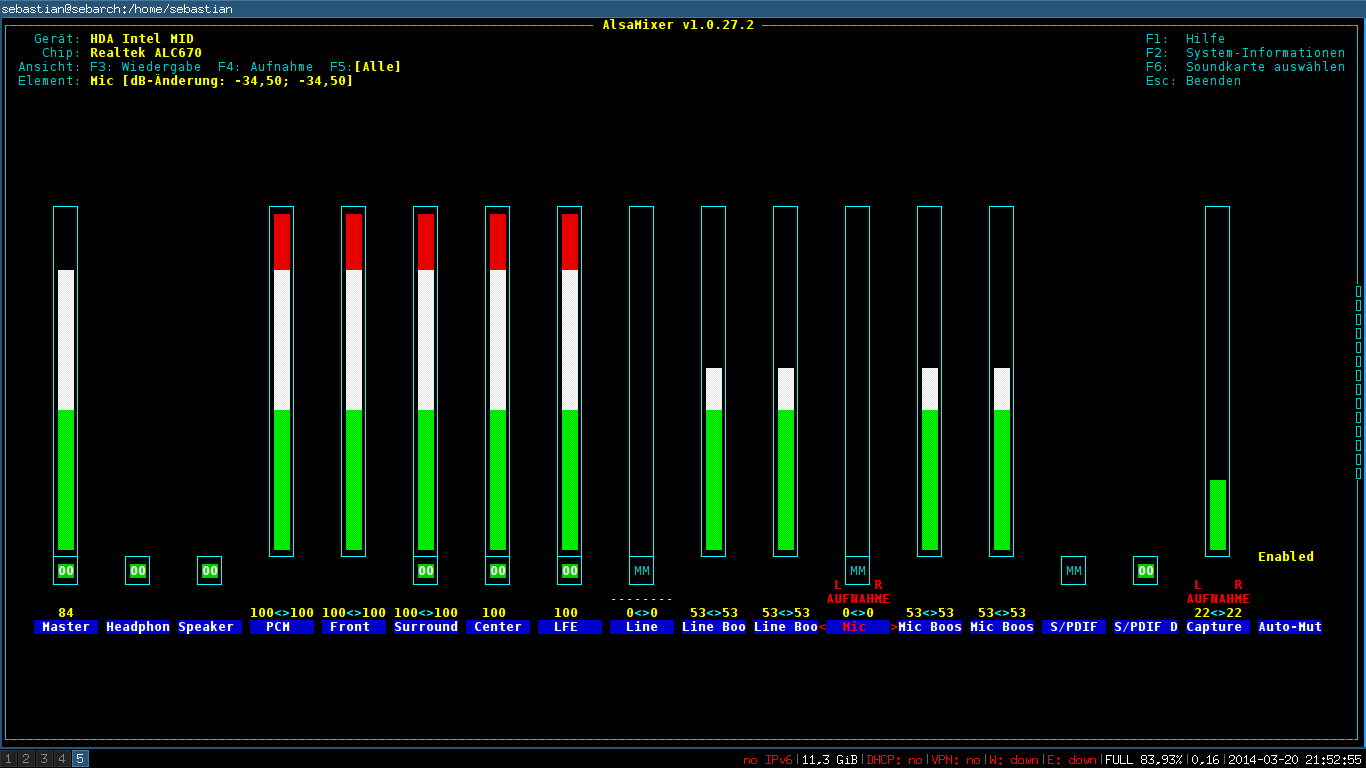
\includegraphics[width=1\textwidth]{alsamixer.png}

\subsection{X11}
\label{sec:x11}
Installiere Xorg-server, Graphikkartentreiber, Windowmanager und Touchpadtreiber:
\begin{lstlisting}[style=Bash]
# pacman -S xorg-server xorg-server-utils xorg-xinit 
# pacman -S mesa xf86-video-ati lib32-ati-dri
# pacman -S i3
# pacman -S xf86-input-synaptics
\end{lstlisting}
Füge ans Ende der \emph{.xinitrc} i3 als wm ein:
\begin{lstlisting}[style=Bash]
$ vi .xinitrc 

...
xrandr --output LVDS --off --output HDMI-0 --auto
exec i3
$
\end{lstlisting}
Wallpaper: 
\begin{lstlisting}[style=Bash]
# pacman -S feh
# systemctl enable cronie
$ crontab -e
...
*/15 * * * * DISPLAY=:0.0 feh --bg-scale /home/sebastian/Bilder/Wallpaper
...
$
\end{lstlisting}
Der X-Server wird gestartet
\begin{lstlisting}[style=Bash]
$ startx
...
$
\end{lstlisting}
